% !TEX root = ../build-polygon/proof-recursion.tex


\section{Introduction}

This document specifies how the polygon zkEVM is proven using 
recursion, agregation and composition.
The constraints of the zkEVM are specified as polynomial identities using the 
PIL language. Then, an execution trace can be proven using the PIL specification for 
building a STARK that is proved with the FRI protocol.
The problem is that STARKs generate big proofs. 
This document describes how to use recursion together with composition to shorten the prove size.

In a high level, a basic recursion block transforms a PIL specification into the 
specification of its STARK verification circuit (written in Circom). 
The circuit verifies the STARK of the PIL specification. 
Then, the Circom specification is transformed into a Plonkish PIL specification and the process is iterated.

In addition to recursion, also aggregation is implemented so that provers 
can aggregate the proofs of multiple transaction batches. 


\ifBACKGROUND
\section{Background}

%%%%%%%%%%%%%%%%%%%%%%%%%%%%%%%%%%%%%%%%%%%%%%%%%%%%%%%%%%%%%%%%%%%
\subsection{SNARK Composition} \label{sec:composition}

Imagine that we have two SNARK proof systems, $\A$ and $\B$, with different cost profiles. For example, assume that the prover in the first $\A$ is very fast, but the proof size is too large and the verification time is so slow to be directly deployed in practise. In contrast, the prover is second $\B$ is really slow, but the proof size is short and the verification time as good as it can be. Even if this looks like a very artificial scenario, this actually happens very often in the real world; where different state-of-the-art SNARKs have different trade-offs and therefore one has to choose the best one, in terms of costs, for his specific use case.

The previous situation depicts the following question: is it possible to combine them in some way to obtain a SNARK that inherits the best costs of both $\A$ and $\B$? More specifically, we want to obtain a SNARK $\C$ with the fast prover of $\A$ and the short proof size and fast verification time of $\B$.

Theoretically, it is possible via \textit{proof composition} which works as follows. Denote by $(\P_X, \V_X)$ the prover and the verifier of some SNARK $X$.  Say that $\P_{\C}$ claims to know a witness for a particular statement. First, $\P_{\C}$ uses $\P_{\A}$ to generate a SNARK proof $\pi$ of the claim. However, since $\pi$ is big and slow to verify, $\P_{\C}$ does not directly send $\pi$ to $\P_{\C}$. Instead, $\P_{\C}$ uses $\B$ to generate a proof $\pi'$ for the following statement:
\begin{center}
	``I know a proof $\pi$ for the original statement that makes $\V_{\A}$ accept with high probability.''
\end{center}
Then, $\P_{\C}$ sends $\pi'$ to $\V_{\C}$. In other words, $\P_{\C}$ uses $\P_{\A}$ to generate a proof $\pi$, then writes down the verification procedure of $\V_{\A}$ as a statement, uses $\P_{\B}$ to generate the proof $\pi'$ and finally uses $\V_{\B}$ to verify $\pi'$. Figure \ref{fig:composition} shows a diagram for this whole process.

It is important to remark here that proof composition requires taking the verification procedure as carried on by $\V_{\A}$ and written down in the underneath computational model used by $\B$. Hence, if arithmetic circuits are used, then one must write the verification part as an arithmetic circuit satisfiability instance.

\begin{figure}[H]
	\centering
	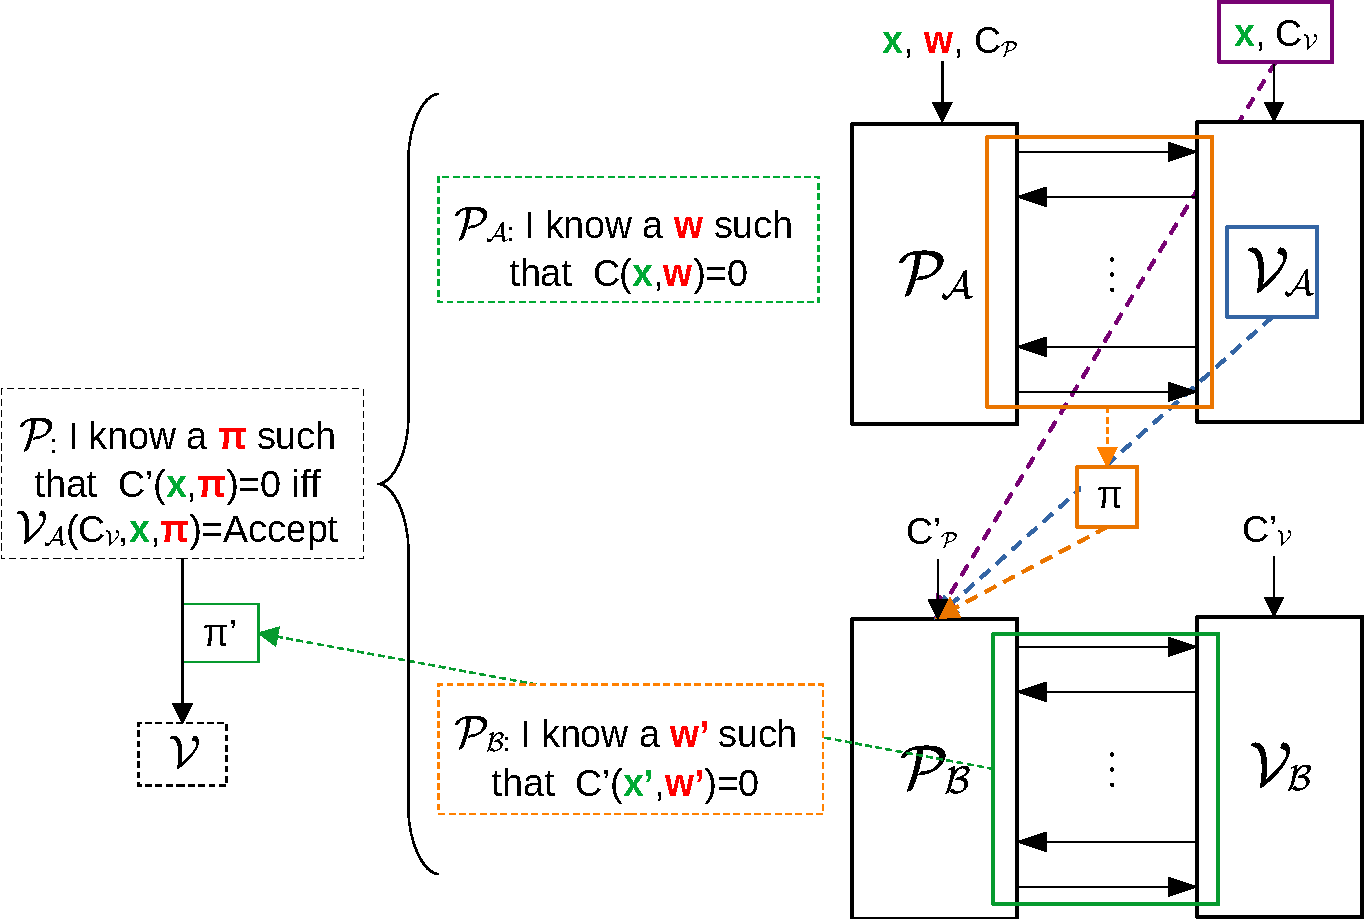
\includegraphics[width=.75\textwidth]{\recursiondir/figures/composition-diagram}
	\caption{Resulting statement obtained from a (depth-$1$) SNARK composition.}
	\label{fig:composition}
\end{figure}

\paragraph*{Costs of the Composition.}
Let's now discuss the costs of $\C$. Since $\P_{\C}$ only sends the second proof $\pi'$ to $\V_{\C}$, the proof size of $\C$ is the size of $\pi'$ as generated by $\V_{\B}$. Moreover, the verification time is precisely the time that $\V_{\B}$ takes to verify $\pi'$. Since the proof size and verification time of $\B$ are short and fast, respectively, the proof size and verification time of $\C$ are short and fast as well.

On the other hand, $\P_{\C}$ first has to generate the proof $\pi$ using $\P_{\A}$, and then has to generate the proof $\pi'$ using $\P_{\B}$. As commented at the beginning of the section, $\P_{\A}$ is fast whereas $\P_{\B}$ is slow. Wouldn't this imply that $\P_{\C}$ is slow? The key point is that the circuit of the verification procedure of $\V_{\A}$ is much more small than the circuit used to compute the first proof, since the verification time taken by $\V_{\A}$ is small (even if not optimal). Hence, the time required by $\P_{\C}$ to generate the second proof $\pi'$ is tiny compared to the time required to compute $\pi$. So, the proving time of $\P_{\C}$ is almost equal to the proving time of $\P_{\A}$, which is fast by assumption.

The best costs of both SNARKs have been achieved.




%%%%%%%%%%%%%%%%%%%%%%%%%%%%%%%%%%%%%%%%%%%%%%%%%%%%%%%%%%%%%%%%%%%
\subsection{Deeper Composition and Proof Recursion}

In the previous section we have seen how SNARK composition looks like and explained it with the generic case of two distinct SNARKs. In this section we explore what happens when we compose a SNARK with itself many times. This procedure is known as \textit{proof recursion}, and its name originates from the resemblance of any computer program being able to be evaluated at itself.

Say that we have a SNARK $\A$ with both proof size and evaluation time of size $O\left(N^{1/2}\right)$. Composing $\A$ with itself yields a new SNARK with proof size and verification time $O\left(\left(N^{1/2}\right)^{1/2}\right) = O\left(N^{1/4}\right)$. One more invocation of $\A$ will yield a new SNARK with proof size and verification time $O\left(N^{1/8}\right)$. One might be attempted to think that this composition can be carried on as many times as he would like, so that proof size and verification time fits with his objectives. However, there exists some upper bound, known as the \textit{recursion threshold}, to the minimum size that can be reached. This threshold refers to the smallest circuit size $N^{\star}$ such that the verification procedure of the initial SNARK $\A$ cannot be represented by a circuit of size smaller than $N^{\star}$. One example of a recursion threshold is the one obtained by Halo \cite{EPRINT:BowGriHop19}, which was proven to be as big as $2^{17}$. Not surprisingly, if one reaches the threshold and instantiate $\A$ another time, not only the resulting SNARK does not reduce costs, but in fact increase them.

What happens with the proving time? Simply put: the more compositions the resulting SNARK is composed of, the more work the prover has to do. Recall from the previous section that the prover must compute one proof per instantiation of the SNARK. For example, if $\A$ is composed with itself three times, the computer first computes a proof $\pi$ that would convice the $\A$ verifier, then produce a proof $\pi'$ that it knows a valid $\pi$, and finally a proof $\pi''$ that it knows a valid $\pi'$. Ever if the consequent proofs take substantially less time than the first one, there is some more work to do that just producing $\pi$.





%%%%%%%%%%%%%%%%%%%%%%%%%%%%%%%%%%%%%%%%%%%%%%%%%%%%%%%%%%%%%%%%%%%
\subsection{Further Applications}

In the previous section we have seen that SNARK composition can be used to improve the overall efficiency of existing SNARKs. Even if complex, this is a generic strategy to improve state-of-the-art SNARKs to whom is unclear if some optimizations are possible, or even when such optimizations are constrained by theoretical bounds. Importantly, applications of proof composition are not restricted to be of efficiency nature. In this section we explore some more applications of proof composition.



\paragraph*{Iterative Computation.} An interesting application of proof recursion is the one of \textit{iterative computation}. In this context, a designated prover $\P$ intends to prove to a verifier $\V$ that for some (public or secret) input $x$ and a publicly known function $f$ we have that:
\[
	f^{(i)}(x) := \underbrace{f(f(\dots f(f}_{i}(x)) \dots)) = y,
\]
where $y$ is a public output. One might notice that applying the same function $f$ some amount of times to an input $x$ is the same as function composition. Hence, one can build SNARKs for iterative computation by generating a SNARK of a single iteration of $f$ on $x$ and then composing the SNARK with itself the requested number of times.

\paragraph*{Incrementally Verifiable Computation.} A generalization of iterative computation is \textit{incrementally verifiable computation}. The idea is that, after each iteration $i$ of $f$ on $x$, $\P$ is able to output a partial computation $y_i$ and a proof $\pi_i$ that $f^{(i)}(x) = y_i$. Then, possibly before performing another iteration, a verifier is able to check the proof $\pi_i$ and be sure with high probability that $f$ has been correctly applied up until this point. Moreover, any party can resume the computation from that point and still be able to generate subsequent proofs.

\paragraph*{Proof Aggregation.} \textit{Proof aggregation} is a particular type of proof composition in which multiple valid proofs can be all proven to be valid by comprising them all into one proof, called the \textit{aggregated proof}, and only validating the aggregated one. More formally, $T$ parties (possibly the same one) $\P_1, \dots, \P_T$ use some proof system to produce proofs $\pi_1, \dots, \pi_T$. Then, instead of having one verification procedure per each proof, composition is used to prove the following statement:
\begin{center}
	I know valid proofs $\pi_1, \dots, \pi_T$ such that $C(\pi_1, \dots, \pi_T) = 0$,
\end{center}
where $C$ is the arithmetic circuit representing the verification procedure of all $\pi_1, \dots, \pi_T$.

The notion of proof aggregation becomes useful in the context of distributed computation, where a computation is too heavy to be carried out by a single party. Instead, the party would break the computation in $T$ pieces and send each of these pieces to a different party, who would produce a proof along with the output of each part. Finally, the original party would combine all the pieces into the actual output and produce a proof of the whole computation.


\paragraph*{Application to Blockchain Scalability.} Some mentioned applications could be combined to achieve \textit{scalability of blockchains}. That is, in order for a blockchain to improve its throughput (i.e., number of transactions per second), which is typically limited by block size and block finding speed, one can choose to perform transactions off-chain and publish a proof of correct state evolution on-chain.

There are several ways of accomplishing the off-chain proof. One can go for computing a proof of a blockchain's state update due to transactions within a block and then simply verify the proof on-chain. Even if totally possible, this is not the lowest cost solution since a blockchain's scalability solution must consume as less storage and verification time as possible. Because of these objectives, a more appropriate proof management design can be obtained using proof composition and/or proof aggregation.
Figure \ref{fig:composition-blockchain} provides a possible proof-management design through a combination of both proof techniques.
\begin{figure}[H]
	\centering
	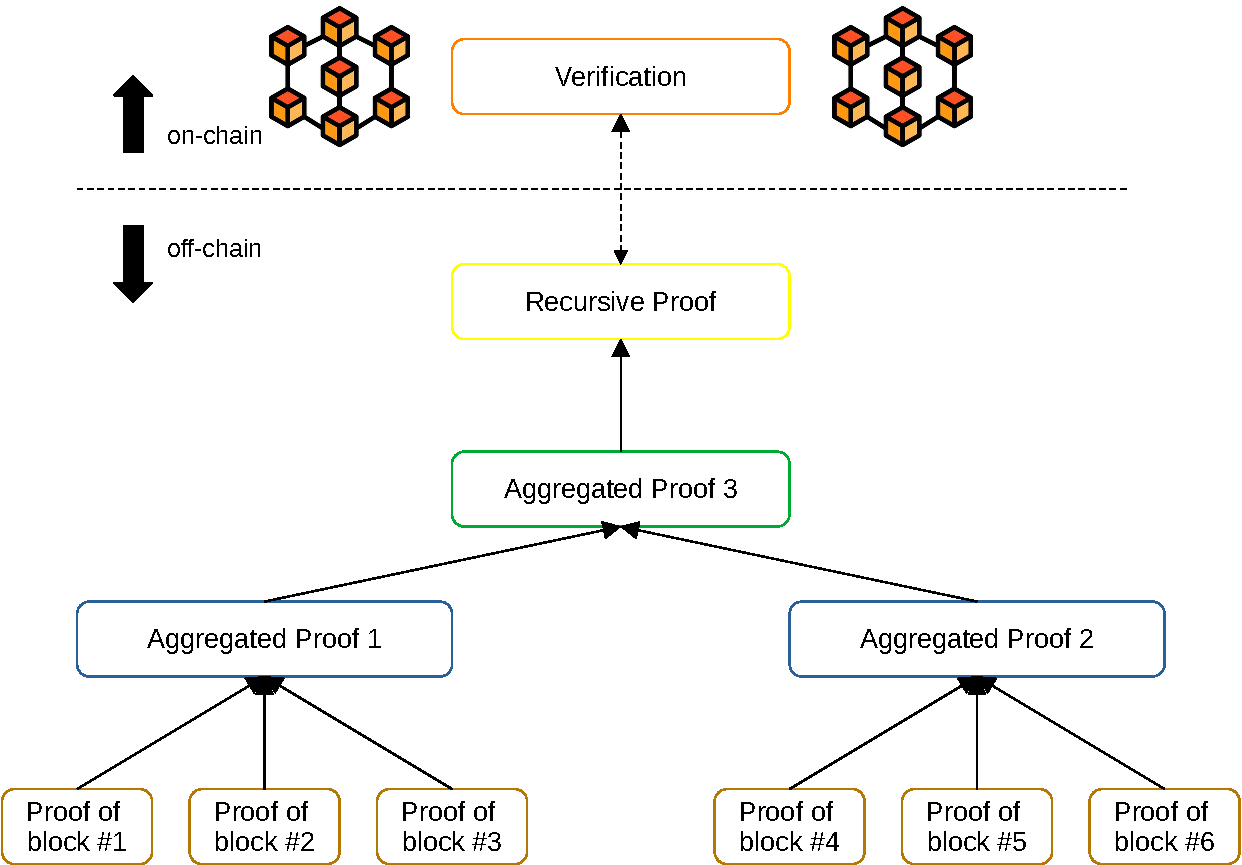
\includegraphics[width=.7\textwidth]{\recursiondir/figures/composition-blockchain}
	\caption{Design candidate's diagram of a proving scheme for the blockchain scalability issue.}
	\label{fig:composition-blockchain}
\end{figure}
As it can be observed, there is a trade-off between the number of blocks to aggregate and time required to perform such proofs. Finding the best scheme for off-chain proving is still an active area of research since there are many variables that come into the place. Which SNARKs to choose, how to combine them efficiently or how to organize the proof generalization are still open questions for those technologies building on top of thes ideas.

The prominent realization of this idea are \textit{rollups} \cite{Thibault2022}, \cite{Lavaur2022}. Section \ref{sec:scalability} will develop on the details about the core ideas of rollups.



%%%%%%%%%%%%%%%%%%%%%%%%%%%%%%%%%%%%%%%%%%%%%%%%%%%%%%%%%%%%%%%%%%%
\subsection{What about Zero-Knowledge?}

There is a good reason why zero-knowledge has not been discuseed up until this point in the whole section. The key fact is that the resulting composed SNARK satisfies the zero-knowledge property if and only if the last SNARK in the composition satisfies it. More exemplified, if $\B$ satisfies zero-knowledge, then so the composition of any other (and any number) SNARK with $\B$ as long as $\B$ is computed the last.

Hence, here we encounter a new potential benefit of proof composition: composing a highly efficient but not zero-knowledge SNARK $\A$ with a zero-knowledge SNARK $\B$ yields a zero-knowledge (and probably highly efficient) SNARK $\C = \B \circ \A$. 

\fi
